% \documentclass[review]{elsarticle}
\documentclass[utf8, babel, sor, jor, amsmath, amssymb, reprint]{elsarticle} %удалить перед отправкой
\usepackage[T2A]{fontenc} %удалить перед отправкой
\usepackage[utf8x]{inputenc} %удалить перед отправкой
\usepackage[english,russian]{babel} %удалить перед отправкой
\graphicspath{{images/}}

\usepackage{lineno,hyperref}
\usepackage{algorithm}
\usepackage{algorithmic}
\modulolinenumbers[5]

\journal{Journal of \LaTeX\ Templates}

\bibliographystyle{elsarticle-num}

\usepackage{mathrsfs}
\usepackage{amsmath}
\usepackage{amssymb}%
\usepackage{multirow}



%%%%%%%%%%%%%%%%%%%%%%%
%% Elsevier bibliography styles
%%%%%%%%%%%%%%%%%%%%%%%
%% To change the style, put a % in front of the second line of the current style and
%% remove the % from the second line of the style you would like to use.
%%%%%%%%%%%%%%%%%%%%%%%

%% Numbered
%\bibliographystyle{model1-num-names}

%% Numbered without titles
%\bibliographystyle{model1a-num-names}

%% Harvard
%\bibliographystyle{model2-names.bst}\biboptions{authoryear}

%% Vancouver numbered
%\usepackage{numcompress}\bibliographystyle{model3-num-names}

%% Vancouver name/year
%\usepackage{numcompress}\bibliographystyle{model4-names}\biboptions{authoryear}

%% APA style
%\bibliographystyle{model5-names}\biboptions{authoryear}

%% AMA style
%\usepackage{numcompress}\bibliographystyle{model6-num-names}

%% `Elsevier LaTeX' style
\bibliographystyle{elsarticle-num}
%%%%%%%%%%%%%%%%%%%%%%%


\usepackage{xcolor}
\newcommand{\todo}[1] {\textcolor{red}{#1}} %%for TODO comments
\def\l{\left\langle}
\def\r{\right\rangle}
\usepackage{mathrsfs}
\usepackage{amsmath}
\usepackage{amssymb}%

\begin{document}

\begin{frontmatter}


\title{Ground state search 2D Ising model}

\author[mainaddress, secondaryaddress]{Viacheslav Trukhin\corref{mycorrespondingauthor}}
\ead{trukhin.vo@dvfu.ru}

\author[mainaddress]{Egor Prokhorov\corref{mycorrespondingauthor}}
\ead{prokhorov.ei@dvfu.ru}

\author[mainaddress, secondaryaddress]{Konstantin Nefedev\corref{mycorrespondingauthor}}
\ead{nefedev.kv@dvfu.ru}


\address[mainaddress]{Far Eastern Federal University, Vladivostok, Russky Island, 10 Ajax Bay, 690922, the Russian Federation}
\address[secondaryaddress]{Institute of Applied Mathematics, Far Eastern Branch, Russian Academy of Science, Vladivostok, Radio 7, 690041, the Russian Federation}

\begin{abstract}


\end{abstract}


\begin{highlights}
	\item Энергия, энтропия и спиновый избыток основного состояния рассчитаны точно методом исчерпывающего перечисления для $10 \times 10$ спинов Изинга на квадратной решетке с открытыми граничными условиями
	\item Влияние размерного эффекта на энтропию и энергию основного состояния вычислено точно, рассчитано асимптотическое поведение энтропии
	\item Явление макроскопического вырождения основного состояния обусловлено наличием кластеров с фрустрированных петлями
	\item Магнитный структурный фактор для разных конфигураций основного состояния
\end{highlights}


\begin{keyword}
	Ising model, GPU and CPU high performance calculations, spin ice, spin glass, statistical thermodynamics.
\end{keyword}


\end{frontmatter}

\linenumbers
\newpage
\tableofcontents

\newpage
\section{Введение}

Всего несколько процентов имеющих магнитный момент атомов, случайно распределенных в немагнитном носителе, таком, например, как благородный металл  \cite{finkler1989spin}, образуют спиновое стекло \cite{belokon2006spin}, которое позволило получить множество интересных экспериментальных результатов. Эти результаты положили начало целому ряду новых тем научных исследований, в частности, в области статистической механики и физики конденсированных сред.

Модель Эдвардса-Андерсона (ЕА) спинового стекла Изинга является одним из простейших примеров моделей спиновых стекол с короткодействующими взаимодействиями. Несмотря на кажущуюся простоту, свойства этой модели для 2D и более высоких размерностей до сих пор не очень хорошо изучены, и даже многие из ее важнейших свойств при Т=0 неизвестны \cite{pal1996ground}. Свойства основного состояния модели Изинга различных решеток с конкурирующими ферромагнитными и антиферромагнитными взаимодействиями изучаются на протяжении множества лет \cite{lebrecht2004plaquette, valdes2012j, lebrecht2015j}. 

В настоящее время модель Изинга актуальна не только в области физики твердого тела, но также находит применение в нейробиологии, моделировании опухолей и описании критических газожидкостных явлений. Несмотря на многие годы интенсивных исследований, природа низкотемпературной фазы модели Изинга фрустрированных спиновых систем с ограниченным радиусом взаимодействия остается невыясненной \cite{newman2023proof}. Два наиболее важных открытых вопроса касаются свойств спиновых стекол при нулевой температуре, в частности, число основных состояний и природа низкоэнергетических возбуждений \cite{newman2022ground}.  

Расчет конфигураций основного состояния спинового стекла с заданным Гамильтонианом является одной из самых сложных оптимизационных задач. В трехмерном случае задача является $NP$-трудной \cite{barahona1982computational, hartmann2002optimization}, что означает ни один известный алгоритм не может решить задачу поиска основного состояния за время, пропорциональное степени линейного размера системы, и считается, что такой алгоритм не может быть разработан. В настоящее время алгоритма, обладающего одновременно высокой точностью и эффективностью, не существует \cite{fan2023searching}.

Изучение спиновых стекол является активной и противоречивой областью статистической физики. В частности, свойства спиновых стекол при нулевой температуре интенсивно изучаются приближенными методами \cite{perez2012ground}. В настоящее время разрабатываются различные приближенные подходы для решения моделей спиновых систем \cite{farias2024differentiable, rybin2022hybrid, makarova2023canonical}. 

Модели спиновых систем на решетках представляют собой идеальную платформу для исследования сложных магнитных основных состояний с возбуждениями, что чрезвычайно важно для физики конденсированного состояния и материаловедения \cite{lacroix2011introduction}. В т.ч. исследования критический полей переключения между основными состояниями, скачков энтропии при переключениях между основными состояниями, корреляционных функций \cite{ramirez2004effect, rosas2004random, andriushchenko2019large}. Попытки приближенного вычисления энергии основного состояния и энтропии в модели спинового стекла Эдвардса-Андерсона на плоской решетке предпринимались \cite{perez2012ground}, однако даже в приближении задача двумерной плотности низкоэнергетическом состояний является трудноразрешимой. Для некоторых решеток, например, для треугольной, все же удается получить информацию об энтропийных и магнитных свойствах \cite{jurvcivsinova2024classical}.

Исследование энергетического ландшафта низкоэнергетических состояний является актуальной задачей \cite{biswas2023energy}. Интересный вопрос касается того, при какой концентрации ферромагнитных обменных взаимодействий относительно концентрации антиферромагнитных обменных будет наблюдаться переход между состоянием (анти-)ферромагнетизма и состоянием спинового стекла \cite{zimmer2022role}. Термодинамические свойства и фазовая диаграмма основного состояния относительно небольшого числа спинов молекулярных кластеров рассчитаны в работе \cite{dias2023ground}.

Конфигурации основных состояний, а также возбуждения в основных и низкоэнергетических конфигурациях искусственного спинового льда, наряду с макроскопическим вырождением основного состояния и остаточной энтропией  при низких температурах активно исследуются в модели дальнодействующего дипольного взаимодействия \cite{makarova2021low, singh2024micromagnetic}.

Задача оценки энергии основного состояния, а также выяснение природы его макроскопического вырождения являются открытыми множество лет. При низких температурах спиновое стекло в основном состоянии проявляет свойства, которые доминируют в его температурном поведении. Пока точного решения не получено, а данные, которые приводятся в литературе, весьма противоречивы. Для $N\rightarrow \infty$ оценки энергии основного состояния различными методами (таб. \ref{tab:Egs}):

\begin{table}[!h]
	\begin{tabular}{|l|c|l|}
		\hline
		Method                                   & $E_{gs}$                                       & ссылка                                          \\ \hline
		Thouless-Anderson-Palmer (TAP) Approach & 0                                              & \cite{thouless1977solution}    \\ \hline
		Replica Method                            & $-2/\pi$                                       & \cite{sherrington1975solvable} \\ \hline
		Partition function                      & -0.5                                           & \cite{tanaka1980analytic}      \\ \hline
		Mean random field                       & $-1/\sqrt{2\pi}$                               & \cite{klein1976comparison}     \\ \hline
		Monte-Carlo                             & -0.76                                          & \cite{kirkpatrick1978infinite} \\ \hline
		Algorithm of Shraudorphs-Kamensky        & -1.33                                          & \cite{karandashev2019global}   \\ \hline
		Parallel Tempering   & -1.40193                                       & \cite{palmer1999ground}        \\ \hline
		  Branch-and-Cut Algorithm              & -1.40197                         
		                                        & \cite{campbell2004energy}      \\ \hline
		                                        & -1.4009                                        & \cite{roma2009ground}          \\ \hline
		Parallel tempering Monte-Carlo  & -1.31479                                       & \cite{roma2009ground}          \\ \hline
	\end{tabular}
	\label{tab:Egs}
	\caption{Удельная энергия основного состояния}
\end{table}

Для конечного числа спинов, и энергия основного состояния будет зависеть очень сильно от конкретной реализации нормального распределения $\left\lbrace J_{ij} \right\rbrace $. Для оценки энергии основного состояния системы конечного числа спинов может быть использован алгоритмы, в т.ч. исчерпывающего перечисления \cite{padalko2021parallel}. В настоящей работе предлагается новый подход к вычислению основных состояний модели Эдвардса Андерсона. Мы получили соответствие решение алгоритмом декомпозиции для энергии основного состояния и остаточной энтропии с решением полученным алгоритмом исчерпывающего перечисления.  


Задачи:
TO DO: \\
1. Энергия основного состояния в зависимости от размеров, асимптотическая оценка $E_{gs}(1/N)$ (есть скрипт)\\
2. Энергия основного состояния в зависимости от $E_{gs}(P_+)$  (есть скрипт)\\
3. Энтропия основных состояний в зависимости от размеров и асимптотика $S(1/N)$  (есть скрипт)\\
4. Энтропия основных состояний в зависимости от  $S(P_+)$   (есть скрипт)\\
5. Записать основные правила расстановки фрустраций.\\
6. Установить природу спинового избытка основного состояния \\
7. Исследовать зависимость вырождения основного состояния от количество и распределения кластеров из плакетов.\\
8. Исследовать природу макроскопического вырождения и значения спинового избытка в зависимости от распределения кластеров с возбужденными петлями по размерам. Установить какие кластеры дают наибольший вклад в вырождение. \\
9. Отрисовать МСФ для основных состояний и сравнить их \\
10. Вычислить зависимость основного состояния от числа фрустрированных плакетов (струн)\\
11. Уточнить, что все образцы имели одинаковое число фрустрированных плакетов (струн) 


\section{Решение исчерпывающим перечислением}

Модель спинового стекла Эдвардса-Андерсона представляет собой плоскую решетку Изинга:

\begin{equation}
	E = -\sum J_{ij} S_i S_j + h \sum S_i,
	\label{eq:ising_energy}
\end{equation}

 где обменные интегралы $J$ могут принимать значения +1 или -1 создавая таким образом приближение аморфных материалов

Для решения такой цепочки из трёх спинов статистическая сумма принимает вид:

\begin{equation}
	Z_3 = e^{3\beta - 3\beta h} + 3e^{\beta - h - \beta} + 3e^{\beta h - \beta} + e^{3\beta + 3\beta h}
	\label{eq:stat_3}
\end{equation}


Численно данное метод выражается в алгоритме \ref{alg:addititional_algorithm}:

Присоединим ещё одну цепочку параллельно первой:

!!!!!!!!Расставить обменные интегралы!!!!!!!!!!!!

\begin{equation}
	\label{eq:stat_3_un}
	\begin{alignedat}{2}
	Z_6 = Z_3 e^{\beta  h-\beta }+Z_3 e^{\beta  h-\beta }+Z_3 e^{\beta  h-\beta }+Z_3 e^{3 \beta +3 \beta  h}+ \\
	Z_3 e^{\beta  (-h)-\beta }+Z_3 e^{\beta  (-h)-\beta }+Z_3 e^{\beta  (-h)-\beta }+Z_3 e^{3 \beta -3 \beta  h}
	\end{alignedat}
\end{equation}

В результате получаем статистическую сумму для решетки $3 \times 2$:

\begin{equation}
	\label{eq:stat_3_res}
	\begin{alignedat}{2}
		Z_6 = 6 e^{-5 \beta }+12 e^{-\beta }+2 e^{3 \beta }+e^{9 \beta -6 \beta  h}+6 e^{3 \beta -4 \beta  h}+6 e^{-3 \beta -2 \beta  h}+\\
		9 e^{\beta -2 \beta  h}+6 e^{2 \beta  h-3 \beta }+9 e^{\beta +2 \beta  h}+6 e^{3 \beta +4 \beta  h}+e^{9 \beta +6 \beta  h}
	\end{alignedat}
\end{equation}

Численное решение таким методом выражается в алгоритме \ref{alg:addititional_algorithm}:


\begin{algorithm}[H]
	\textbf{ВХОД:} Размер решетки, распределение обменных констант.\\
	\textbf{ВЫХОД:} Полная плотность состояний.
	\begin{algorithmic}
		\STATE {Рассчитать плотность состояний для первой 1D цепочки}
		\FOR {Количество слоев в решетке\\}
		{
			\STATE {Рассчитать плотность состояний для присоединяемой 1D цепочки}
			\FOR {длина 1D цепи\\}
			{
				\STATE {Рассчитать плотность состояний для получившейся решетки}
			}
			\ENDFOR\\
		}
		\ENDFOR
	\end{algorithmic}
	\caption{Вычисление плотности состояний методом присоединения 1D цепочек.}
	\label{alg:addititional_algorithm}
\end{algorithm}
				
В результате для квадратной решетки $N \times N$ сложность алгоритма полного перебора падает с $2^{N \cdot N}$ до $N \cdot 2^N + (N - 1) \cdot 2^N$. Таким образом прирост производительности для решетки из 9-ти спинов составляет примерно 92\% и на 27 порядков для системы из 100 спинов.


\section{Правила размещения фрустраций}

Для удобства введём несколько терминов.

 Плакет – это минимальная, замкнутая с помощью связей цепь. В рассмотренных далее примерах на квадратной решётке плакеты являются элементарными квадратами. На рисунке \ref{fig:petlya} приведён пример плакета. Знакам \textquotedblleft +\textquotedblright ~и   \textquotedblleft -\textquotedblright ~соответствуют значения обменных интегралов  \textquotedblleft +1\textquotedblright ~и \textquotedblleft -1\textquotedblright ~соответственно.

\begin{figure}[H]
	\centering
	\begin{minipage}{0.3\textwidth}
		\centering
		\resizebox{50px}{50px}{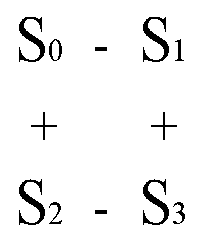
\includegraphics{Petlya.eps}}
		\caption{Плакет}
		\label{fig:petlya}
	\end{minipage}
\end{figure}
Если рассмотреть все возможные комбинации обменных констант в плакете на рисунке \ref{fig:petlya}, то не трудно заметить, что фрустрация в основном состоянии обязательно появляется, если в системе три обменных константы одного знака, а четвёртый другого знака, см. рисунок \ref{fig:struna}. Далее такие плакеты будем называть фрустрированными плакетами.

\begin{figure}[H]
	\centering
\begin{minipage}{0.3\textwidth}
	\centering
	\resizebox{60px}{60px}{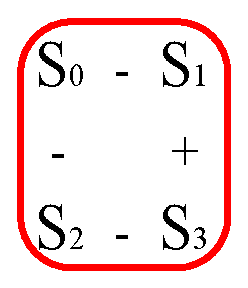
\includegraphics{Struna.eps}}
	\caption{Фрустрированный плакет}
	\label{fig:struna}
\end{minipage}
\end{figure}

Полная энергия взаимодействия спинов во фрустрированном плакете на рисунке \ref{fig:struna}
\begin{equation}
	E = -J_{01} S_0 S_1-J_{02} S_0 S_2-J_{13} S_1 S_3-J_{23} S_2 S_3.
	\label{eq:ising_energy_2x2}
\end{equation}

Всего существует $2^4$ конфигураций, из которых, как показывает метод исчерпывающего перечисления, 8 являются основными состояниями, см. в таблицу \ref{tab:Strunags}. Таким образом, для фрустрированного плакета на рисунке \ref{fig:struna} в основном состоянии каждая из пар спинов может быть фрустрирована.

\begin{table}[H]
		\centering
	\begin{tabular}{|c|c|c|c|}
	
		\hline
	 $S_{gs}$	& $E_{gs}$    & Фрустрация  &   $M_{gs}$   \\
	\hline
	    & & 	$S_2=-1$; $S_3=-1$ & 2   \\ 	\cline{3-4}
	   	& & $S_0=1$,$S_1=1$        & 2\\ 	\cline{3-4}
		& &  $S_1=-1$; $S_3=1$     & 0    \\ \cline{3-4} 
        &  & $S_0=-1$; $S_2=-1$ &	0  \\ 
		\cline{3-4} 
		8	\multirow{3}{*}{} & -2 \multirow{3}{*}{} & $S_1=1$;  $S_3=-1$     &  0\\ \cline{3-4}	
		& & $S_0=1$;  $S_2=1$      &  0\\ \cline{3-4}
		& &	$S_2=1$;  $S_3=1$      &  -2\\ \cline{3-4}
		& &	$S_0=-1$; $S_1=-1$     & -2\\ \hline
	
	\end{tabular}
	\caption{Свойства конфигураций основного состояния фрустрированного плакета на рисунке \ref{fig:struna}}
	\label{tab:Strunags}
\end{table}
  
Тогда логично предположить, что если система состоит из двух фрустрированных плакетов, то для минимизации энергии фрустрированная пара должна быть расположена на пересечении плакетов. На рисунке \ref{fig:3x2}. пример такой системы. Фрустрированной парой спинов будет пара $S_1$,$S_4$.

\begin{figure}[H]
	\centering
	\begin{minipage}{0.3\textwidth}
		\centering
		\resizebox{70px}{70px}{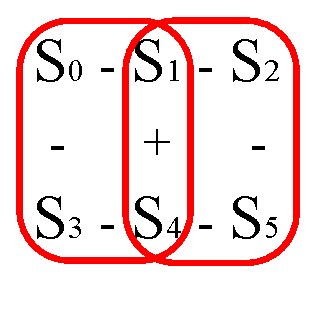
\includegraphics{3x2.eps}}
		\caption{Система состоящая из двух фрустрированных плакетов}
		\label{fig:3x2}
	\end{minipage}
\end{figure}

Метод полного перебора подтверждает правильность данного решения. В Таблице 2 приведены основные состояния данной системы, полученные с помощью полного перебора состояний. Конфигурации спинов в основных состояниях доказывают, что фрустрированной парой является пара $S_1$,$S_4$. 

\begin{table}[H]
	\centering
	\begin{tabular}{|c|c|c|}
		\hline
		 Egs   &   Фрустрированная пара & Mgs\\
		 \hline
		  &  $S_1=1$, $S_4=-1$ & 0 \\
		  \cline{2-3}
		  	-5	\multirow{3}{*}{}
		   &   $S_1=-1$, $S_4=1$ & 0 \\
		\hline
	\end{tabular}
	\caption{Основные состояния системы \eqref{fig:3x2} }
	\label{tab:gs}
\end{table}

Таким образом, зная где расположена фрустрированная пара спинов, а следовательно, и где расположены не фрустрированные пары, можно найти основное состояние системы просто расставляя значение спинов по порядку или начиная с любого спина. 

Примечательно, что расположение фрустрации в подобных системах не зависит от знака обменного интеграла конкретной пары. Главное, чтобы система состояла из двух фрустрированных.


На рисунке \eqref{fig:3x2.2} показан пример другой решётки, состоящей из двух фрустрированных плакетов.

\begin{figure}[H]
	\centering
	\begin{minipage}{0.3\textwidth}
		\centering
		\resizebox{70px}{70px}{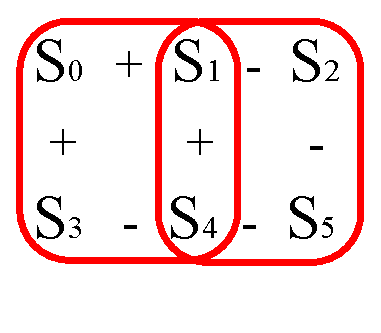
\includegraphics{3x2.2.eps}}
		\caption{Система состоящая из двух фрустрированных плакетов}
		\label{fig:3x2.2}
	\end{minipage}
\end{figure}


\begin{table}[H]
	\centering
	\begin{tabular}{|c|c|c|}
		\hline
		Egs   &   Фрустрированная пара & Mgs \\
		\hline
		   &  $S_1=1$, $S_4=1$ & 2 \\
		\cline{2-3}
		-5	\multirow{3}{*}{}
		 &   $S_1=-1$, $S_4=-1$ & -2 \\
		\hline
	\end{tabular}
	\caption{Основные состояния системы \eqref{fig:3x2.2}}
	\label{tab:gs2}
\end{table}

Несмотря на другие знаки обменных интегралов в таблице \eqref{tab:gs2} видно, что фрустрированной парой также является пара $S_1$,$S_4$.

Также стоит отметить, что на расположение фрустрации в таких системах  не влияют другие плакеты, находящиеся вокруг.

\begin{figure}[H]
	\centering
	\resizebox{180px}{150px}{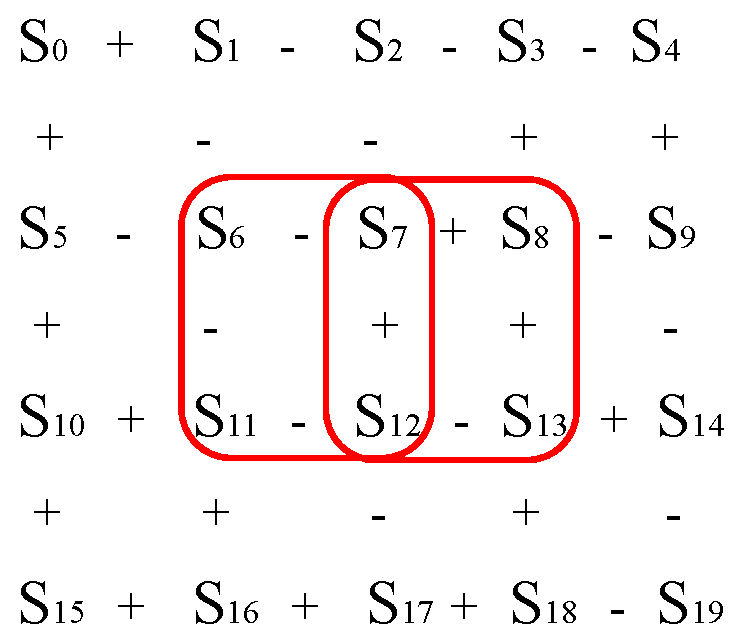
\includegraphics{5x4.eps}}
	\caption{Система из 20 спинов с двумя фрустрированными плакетами в центре}
	\label{fig:5x4}
\end{figure}

На рисунке \eqref{fig:5x4} представлена система из двадцати спинов, в центре которой находятся два фрустрированных плакета, имеющие общую пару спинов. Исходя из предыдущих размышлений, данная система должна обладать одной фрустрированной парой  $S_7$,$S_12$.

\begin{table}[H]
	\centering
	\begin{tabular}{|c|c|c|}
		\hline
		Egs   &   Фрустрированная пара & Mgs\\
		\hline
		 &  $S_7=1$, $S_{12}=1$ & 8 \\
	\cline{2-3}
		-29	\multirow{3}{*}{}
		  &   $S_7=-1$, $S_{12}=-1$ & -8 \\
		\hline
	\end{tabular}
	\caption{Основные состояния системы \eqref{fig:5x4}}
	\label{tab:gs3}
\end{table}

Поиск основных состояний методом исчерпывающего перечисления подтверждает правильность рассуждений \eqref{tab:gs3}.

Если рассматриваемые плакеты пересекаются с несколькими плакетами одновременно, то они формируют кластер.

В кластере необходимо выбрать фрустрированными пары, находящиеся на пересечении так чтобы такая пара была в плакете только одна. Если в каком-то состоянии фрустрированный плакет остался без выбранной пары в силу невозможности её расположения на пересечении плакетов, выбирается одна из трёх оставшихся в плакете пар, по возможности та, которая не будет возбуждать другие плакеты, не входящие в кластер. Это можно сделать с помощью полного перебора состояний пар, где состояние пары может принимать только два значения: пара фрустрирована и пара не фрустрирована.

\begin{figure}[H]
	\centering
	\resizebox{150px}{75px}{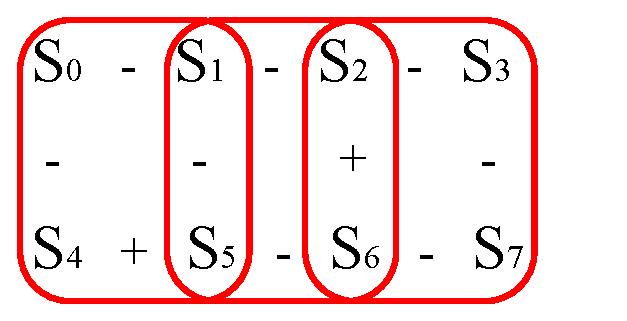
\includegraphics{4x2.eps}}
	\caption{Кластер, состоящий из трёх фрустрированных плакетов}
	\label{fig:cluster}
\end{figure}

В системе \eqref{fig:cluster}  можно выбрать фрустрированной пару $S_1$,$S_5$, тогда пару  $S_2$,$S_6$ выбрать уже нельзя. Второй фрустрированной парой можно выбрать оду из трёх оставшихся в подсистеме пар: $S_2$,$S_3$, $S_3$,$S_7$ или $S_6$,$S_7$. Если изначально выбирается пара $S_2$,$S_6$, то второй будет пара $S_0$,$S_1$, $S_0$,$S_4$ или $S_4$,$S_5$. Далее для каждой из конфигураций фрустраций в системе расставляются значения спинов. Таким образом для данной системы получается 12 основных состояний. 

Полный перебор состояний данной системы подтверждает правильность расстановки фрустраций, энергию и кратность вырождения.

\begin{table}[H]
	\centering
	\begin{tabular}{|c|c|c|}
		\hline
		Egs   &   Фрустрированная пара & Mgs\\
		\hline
		  &  $S_1=1$, $S_5=1$ & \\
		      &    $S_2=-1$, $S_3=-1$ &0 \\
		 \cline{2-3}
		   &  $S_1=1$, $S_5=1$ &\\
		      &    $S_3=1$, $S_7=1$ & 2\\
		 \cline{2-3}
		   &  $S_1=1$, $S_5=1$ & \\
		      &    $S_6=-1$, $S_7=-1$ & 0\\
		 \cline{2-3}
		  &  $S_2=1$, $S_6=-1$ & \\
				&    $S_4=-1$, $S_5=1$ & 0\\
		 \cline{2-3}
		  &  $S_2=1$, $S_6=-1$ &\\
				&    $S_0=-1$, $S_1=-1$ & 0\\
		 \cline{2-3}
		   &  $S_2=1$, $S_6=-1$ &\\
				&    $S_0=1$, $S_4=1$ & 2\\
				\cline{2-3}
				-6	\multirow{3}{*}{}
		   &  $S_1=-1$, $S_5=-1$ &\\
			&    $S_2=1$, $S_3=1$ & 0\\
		\cline{2-3}
		   &  $S_1=-1$, $S_5=-1$ &\\
			&    $S_3=-1$, $S_7=-1$ & -2\\
		\cline{2-3}
		   &  $S_1=-1$, $S_5=-1$ &\\
			&    $S_6=1$, $S_7=1$ & 0\\
	\cline{2-3}
		   &  $S_2=-1$, $S_6=1$ &\\
			&    $S_4=1$, $S_5=-1$ & 0\\
	\cline{2-3}
		   &  $S_2=-1$, $S_6=1$ &\\
			&    $S_0=1$, $S_1=1$ & 0\\
		\cline{2-3}
		   &  $S_2=-1$, $S_6=1$ &\\
			&    $S_0=-1$, $S_4=-1$ & -2\\
		\hline
	\end{tabular}
	\caption{Основные состояния кластера \eqref{fig:cluster}}
	\label{tab:gs_cl}
\end{table}


\begin{figure}[H]
	\centering
	\resizebox{150px}{150px}{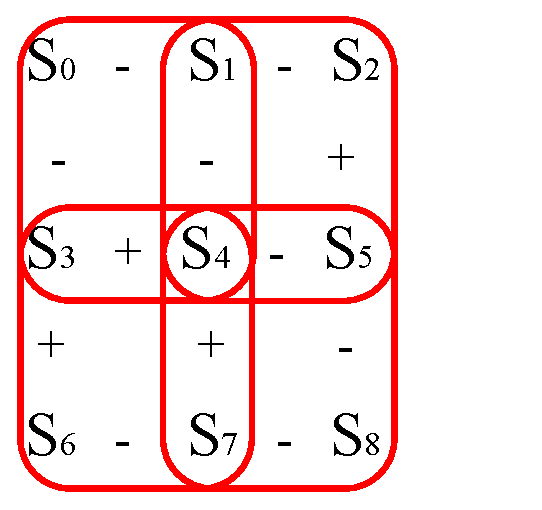
\includegraphics{3x3.eps}}
	\caption{Кластер, состоящий из четырёх фрустрированных плакетов}
	\label{fig:3x3}
\end{figure}

В кластере, состоящем из четырёх фрустрированных плакетов \ref{fig:3x3} все фрустрированные пары расположены на пересечениях.

\begin{table}[H]
	\centering
	\begin{tabular}{|c|c|c|}
		\hline
		Egs   &   Фрустрированная пара & Mgs\\
		\hline
		   &  $S_3=1$, $S_4=-1$&\\
		&    $S_4=-1$, $S_5=-1$ & -1\\
	\cline{2-3}
		   &  $S_1=1$, $S_4=1$&\\
		&    $S_4=1$, $S_7=-1$ & 1\\
			\cline{2-3}
		-8	\multirow{3}{*}{}
		  &  $S_3=-1$, $S_4=1$&\\
			&    $S_4=1$, $S_5=1$& 1\\
		\cline{2-3}
		   &  $S_1=-1$, $S_4=-1$&\\
			&    $S_4=-1$, $S_7=1$& -1\\
		\hline
	\end{tabular}
	\caption{Основные состояния кластера \ref{fig:3x3}}
	\label{tab:gs_3x3}
\end{table} 

\begin{figure}[H]
	\centering
	\resizebox{150px}{100px}{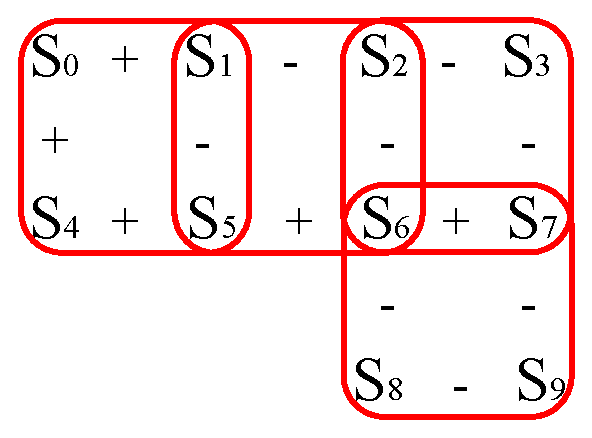
\includegraphics{4cl.eps}}
	\caption{Кластер, состоящий из четырёх фрустрированных плакетов}
	\label{fig:cl}
\end{figure}

\begin{figure}[H]
	\centering
	\resizebox{150px}{100px}{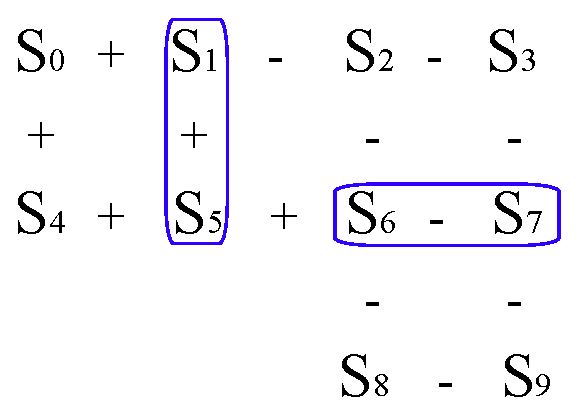
\includegraphics{4clF.eps}}
	\caption{Кластер, в котором отмечены фрустрированные в основном состоянии пары спинов}
	\label{fig:clF}
\end{figure}

\begin{table}[H]
	\centering
	\begin{tabular}{|c|c|c|}
		\hline
		E   &   Фрустрированная пара & Mgs\\
		\hline
		   &  $S_1=1$,$S_5=1$&\\
		&    $S_6=1$,$S_7=-1$ & 4\\
	\cline{2-3}
		-9	\multirow{3}{*}{}
		   &  $S_1=-1$,$S_5=-1$&\\
		&    $S_6=-1$,$S_7=1$ & -4\\
		\hline
	\end{tabular}
	\caption{Основные состояния кластера \ref{fig:3x3}}
	\label{tab:gscl}
\end{table} 

В реальных системах кластеры могут иметь не такую простую форму, например, как на рисунке \ref{fig:cl}. Фрустрированные пары в данном кластере также располагаются по такому же принципу (рисунок \ref{fig:clF}, таблица \ref{tab:gscl}).


\begin{figure}[H]
	\centering
	\resizebox{150px}{150px}{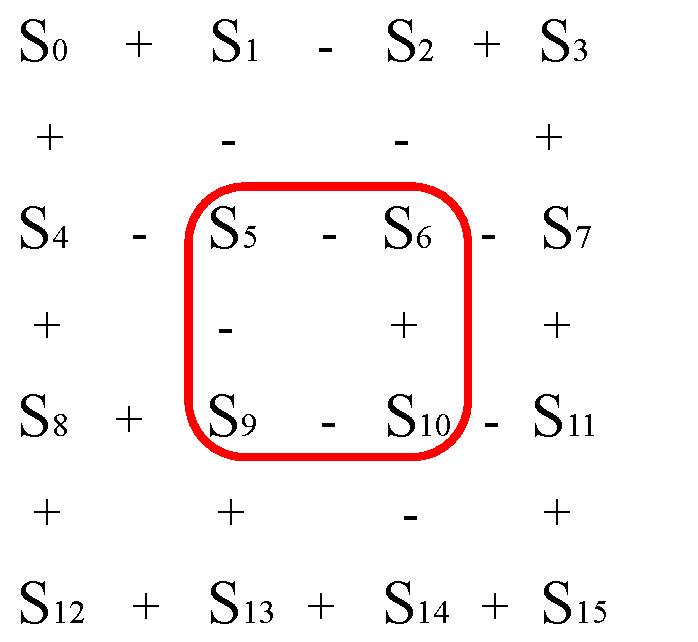
\includegraphics{4x4.eps}}
	\caption{Система, состоящая из фрустрированного плакета, окружённого другими плакетами}
	\label{fig:4x4}
\end{figure}

Если фрустрированный плакет не образует кластер, но при этом всё же пересекается с другими плакетами как на рисунке \ref{fig:4x4}, то какую бы пару во фрустрированном плакете мы не посчитали фрустрированной она будет возбуждать соседний плакет также делая её фрустрированным и в ней будет появляться вторая фрустрация причём таким, образом чтобы не возбуждать другие плакеты. 

\begin{table}[H]
	\centering
	\begin{tabular}{|c|c|c|}
		\hline
		Egs   &   Фрустрированная пара & Mgs \\
		\hline
		  &  $S_5=1$, $S_6=1$& \\
		&    $S_1=-1$, $S_2=-1$ & -10\\
		\cline{2-3}
		   &  $S_5=1$, $S_9=1$& \\
		&    $S_4=-1$, $S_8=1$& 6\\
			\cline{2-3}
		  &  $S_6=1$, $S_{10}=-1$&\\
		&    $S_7=-1$, $S_{11}=1$& 6\\
		\cline{2-3}
		   &  $S_9=1$, $S_{10}=1$&\\
		&    $S_{13}=1$, $S_{14}=-1$& 2\\
		\cline{2-3}
		-20	\multirow{3}{*}{}
		  &  $S_5=-1$, $S_6=-1$&\\
		&    $S_1=1$, $S_2=1$& 10\\
		\cline{2-3}
		  &  $S_5=-1$, $S_9=-1$&\\
		&    $S_4=1$, $S_8=-1$& -6\\
		\cline{2-3}
		   &  $S_6=-1$, $S_{10}=1$&\\
		&    $S_7=1$, $S_{11}=-1$& -6\\
			\cline{2-3}
		  &  $S_9=-1$, $S_{10}=-1$&\\
		&    $S_{13}=-1$, $S_{14}=1$& -2\\
		\hline
	\end{tabular}
	\caption{Основные состояния системы \ref{fig:4x4}}
	\label{tab:gs_4x4}
\end{table}

\begin{figure}[H]
	\centering
	\resizebox{150px}{150px}{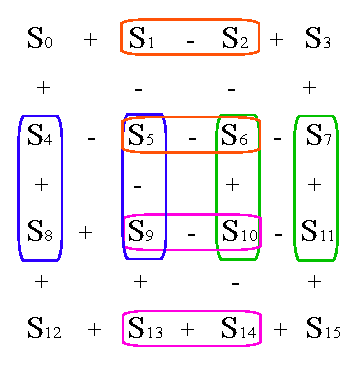
\includegraphics{4x4.1.eps}}
	\caption{Система \ref{fig:4x4}, в которой отмечены фрустрированные пары спинов в основных состояниях. Разные цвета соответствуют разным основным состояниям}
	\label{fig:4x4.1}
\end{figure}

Основные состояния данной системы, полученные полным перебором \ref{tab:gs_4x4}, подтверждают, что одна фрустрированная пара находится во фрустрированном плакете, а вторая в соседнем так, чтобы не пересекаться с другими плакетами, то есть с краю \ref{fig:4x4.1}.

\begin{figure}[H]
	\centering
	\resizebox{200px}{150px}{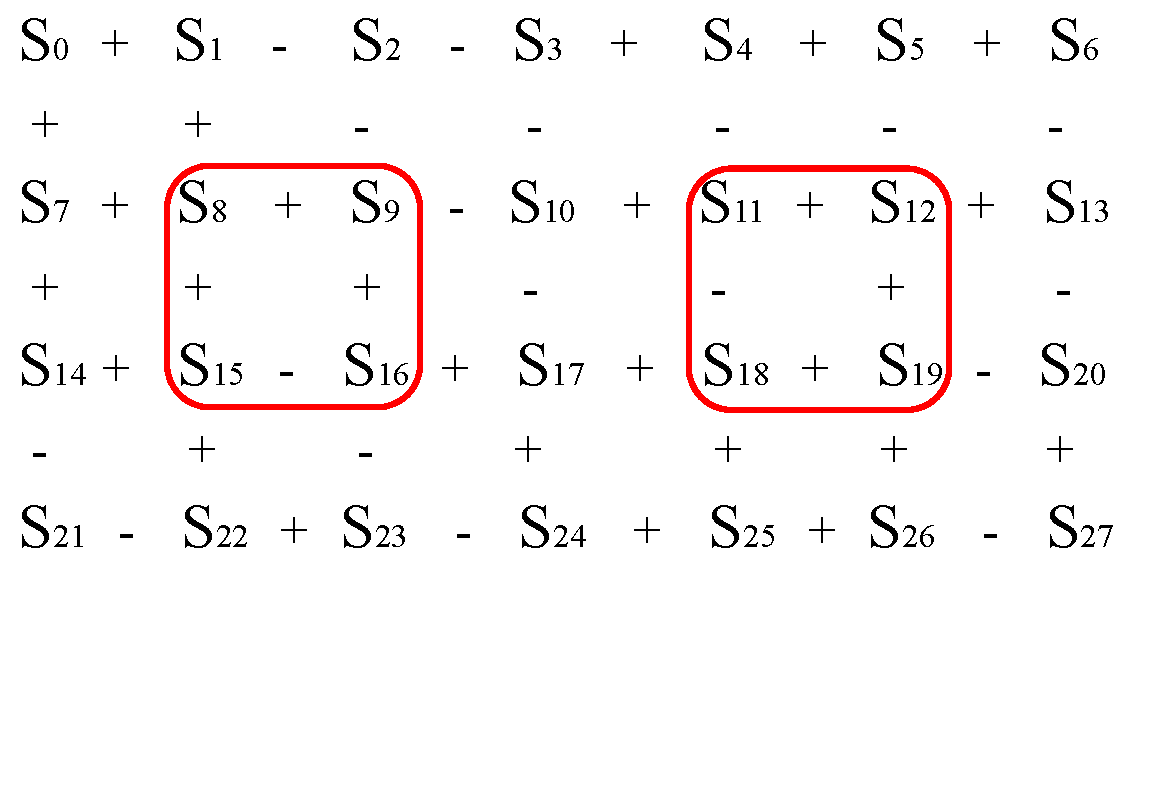
\includegraphics{4x7.eps}}
	\caption{Система, обладающая двумя непересекающимися фрустрированными плакетами}
	\label{fig:4x7}
\end{figure}
\begin{figure}[H]
	\centering
	\resizebox{200px}{150px}{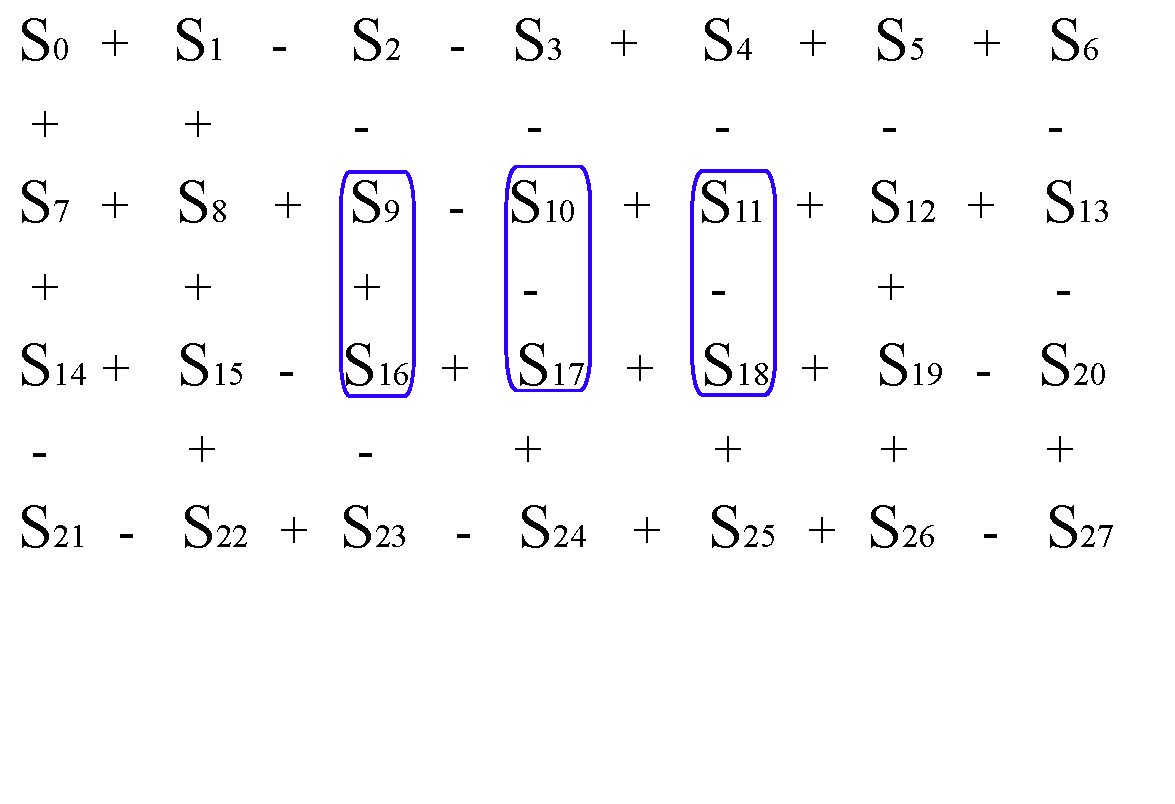
\includegraphics{4x7F.eps}}
	\caption{Система \ref{fig:4x7}, на которой отмечены фрустрированные пары  в основных состояниях.}
	\label{fig:4x7F}
\end{figure}

Если в системе два непересекающиеся фрустрированных плакета \ref{fig:4x7}, то возможна такая ситуация, что им энергетически выгоднее возбуждать плакеты по направлению друг к другу \ref{fig:4x7F}.

\begin{figure}[H]
	\centering
	\resizebox{150px}{150px}{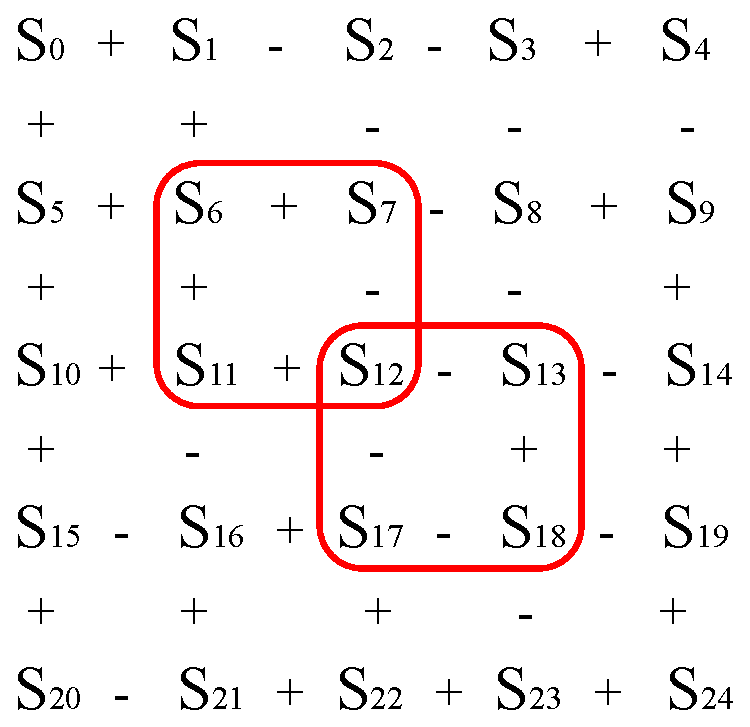
\includegraphics{5x5.2F.eps}}
	\caption{Система, обладающая двумя фрустрированными плакетами, имеющими один общий спин}
	\label{fig:5x5.2F}
\end{figure}
\begin{figure}[H]
	\centering
	\resizebox{150px}{150px}{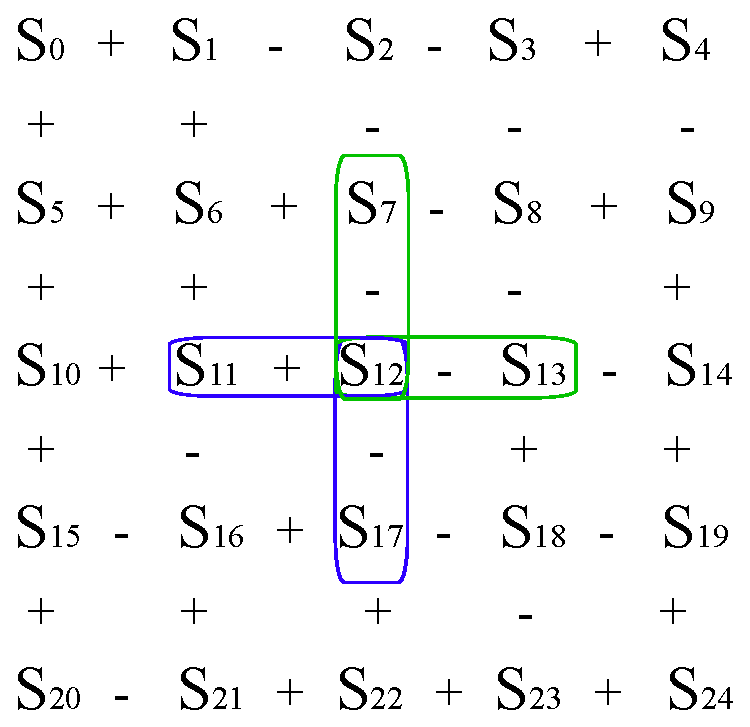
\includegraphics{5x5.2F2.eps}}
	\caption{Система \ref{fig:5x5.2F}, в которой отмечены фрустрированные пары спинов в основных состояниях. Разные цвета соответствуют разным основным состояниям}
	\label{fig:5x5.22F}
\end{figure}
Также стоит рассмотреть случай, когда два фрустрированных плакета имеют лишь один общий спин \ref{fig:5x5.2F}.
В таком случае фрустрации будут располагаться так, чтобы возбуждать один и тот же соседний плакет.
Метод исчерпывающего перечисления подтверждает расположение фрустраций.

На основе рассмотренных примеров можно сделать несколько выводов: \\
1. Фрустрированные плакеты являются единственным источником возниконовения фрустраций в основном состоянии.\\
2. Погасить возбуждение идущие от фрустрированного плакета можно с помощью другого фрустрированного плакета или с помощью края решётки, в заивисимости от расстояний.

Далее исходя из выводов был сформулирован алгоритм по поиску основного состояния

\begin{algorithm}[H]
	\small
	\centering
	\textbf{ВХОД:} Размер решетки, распределение обменных констант.\\
	\textbf{ВЫХОД:} Конфигурация спинов в основном состоянии.\\
	\begin{algorithmic}
		\STATE {Сгруппировать все возможные плакеты из номеров спинов\\}
		\STATE {Присвоить плакетам координаты x,y\\}
		\STATE {Определить фрустрированные плакеты\\}
		\STATE {Вызов функции \\}
		\STATE {Функция\\
		}
		{
		\IF {Плакеты сгруппированы по парам\\}
		{\FOR {Количество пар плакетов\\}
		{\STATE {Рассчитываем количество фрустрированных пар спинов от одного плакета до другого с помощью координат плакетов\\}
		\STATE {Рассчитвыаем количество фрустрированных пар от плакетов до ближайших к ним краёв решётки\\}
		\STATE {Выбираем меньшую из двух вычисленных величин\\}
		\STATE {Фиксируем фрустрации как пары номеров спинов\\}
		}
		\ENDFOR\\
		\STATE {Суммируем количество фрустраций для каждой пары плакетов в комбинации\\}
		\STATE {Сравниваем с количеством фрустраций в предыдущей комбинации и оставляем комбинацию с меньшим числом фрустраций\\}
		}
		\ENDIF\\
		\FOR {Количество фрустрированных плакетов\\}
		{	\IF {текущий плакет не был использован для группировки\\}
			{	\STATE {Плакет помечается как использованный\\}
			\FOR {Количество оставшихся фрустрированных плакетов\\}
			{
			\IF {текущий плакет не был использован для группировки\\}
			{	\STATE {Плакет помечается как использованный\\}
			\STATE	{Из двух помеченных плакетов формируется пара\\}
			\STATE	{Происходит рекурсивный вызов функции для формирования оставшихся пар (цикл начинается со следующего по номеру плакета)\\}}
			\ENDIF\\
			}
			\ENDFOR\\
		}
			\ENDIF\\
		}
		\ENDFOR\\
		}
		\STATE {Для выбранной комбинации с наименьшим числом фрустраций расшифровываем значение спинов\\
		}
		\STATE {Выбираем значение первого спина произвольно (1 или -1)\\
		}
		\FOR {Количество спинов начиная со второго\\}
		{\IF {спин с одиним из предыдущих образуют фрустрированную пару\\}
			{\STATE {Значение спина равно произведению второго спина находящегося с ним во фрустрированной паре, обменному интегралу между ними и минус единице\\}
			}
		\ELSE 
		{\STATE {Значение спина равно произведению второго спина находящегося с ним во фрустрированной паре и обменному интегралу между ними\\}}
		\ENDIF\\}
		\ENDFOR\\
	\end{algorithmic}
	\caption{Вычисление основного состояния перебором комбинаций группировок фрустрированных плакетов по парам.}
	\label{alg:alg_2}
\end{algorithm}

Пояснения к алгоритму:\\
1. Число фрустраций между i,j-той парой плакетов определяется как $\left|x_i-x_j\right|+\left|y_i-y_j\right|$\\
2. Число фрустраций, возникающее от фрустрированного плакета до ближайшего края рештки определяется как $R_{ij}+1$, где i - номер фрустрированного плакета, j - номер ближайшего плакета находящегося на краяю рештки, $R_{ij}$ - расстояние между ними.\\
3. Если в системе нечётное n количество фрустрированных плакетов, то функция вызывается в цикле n раз. На каждой итерации цикла исключаем один из плакетов, который не участвует в комбинировании. Фрустрации от этого плакета распространяются в направлении ближайшего края и также суммируются со всеми остальными в каждой комбинации.\\
4. Количество уникальных комбинаций, которые необходимо рассмотреть для обнаружения основного состояния можно получить из формулы числа неупорядоченных разбиений:
\begin{equation}
	N(m_1,m_2,...,m_n)=\dfrac{n!}{(1!)^{m_1}*(2!)^{m_2}*...*(n!)^{m_n}*m_1!*m_2!*...*m_n!}
	\label{eq:unordered_partitions}
\end{equation}
Тогда для рассматриваемого случая разбиения по парам число возможных комбинаций определяется по формуле:
\begin{equation}
	N(\frac{n}{2})=\dfrac{n!}{2^{\frac{n}{2}}*\frac{n}{2}!}
	\label{eq:unordered_partitions2}
\end{equation}
5. Минусом приведнного алгоритма является то, что он не генерирует исключительно уникальные комбинации. К примеру для системы из четырёх плакетов будут сгенерированы комбинации ${(1,2),(3,4)}$ и ${(3,4),(1,2)}$, которые на самом деле являются идентичными.

Поиски основного состояния показали, что оно может обладать довольно высокой кратностью вырождения. Это происходит по нескольким причинам:\\
1. Различные комбинации фрустрированных плакетов могут давать одинаковое количество фрустраций.\\
2. Распространение возбуждения от одного плакета к другому могут идти по разным тракеториям при этом давая одинаковое количество фрустраций.\\
3. Сумма фрустраций идущих от пары плакетов к ближайшим краям решётки может быть равной количеству фрустраций от одного плакета к другому.\\
4. Для плакета возбуждение от которого идёт к краю решётки может быть несколько краёв находящихся на одинаковом расстоянии.\\

Для исследования основных состояний были взяты 2000 различных решёток спинового стекла.
Размеры решёток были от 8x8 до 32x32. Для каждого размера рассматривались системы с различным чётным количеством фрустрированных плакетов (от 2 до 16) и для каждого количества плакетов было взято по 10 систем со случайной расстановкой фрустрированных плакетов внутри системы. Для исследования не  брались решётки с нечётным количеством плакетов так как тогда невозможно добиться одинакового количества отрицательных и положительных обменных констант. 

Из графика \ref{fig:Egs_N_F} видно что энергия основного состояния системы на один спин увеличивается с числом фрустрированных плакетов. Диапазон таких значений составляет -1.92578 ; -1.34375 , а это значит, что большинство значений меньше чем приведённые в таблице \ref{tab:Egs}. 

\begin{figure}[H]
	\centering
	\resizebox{290px}{220px}{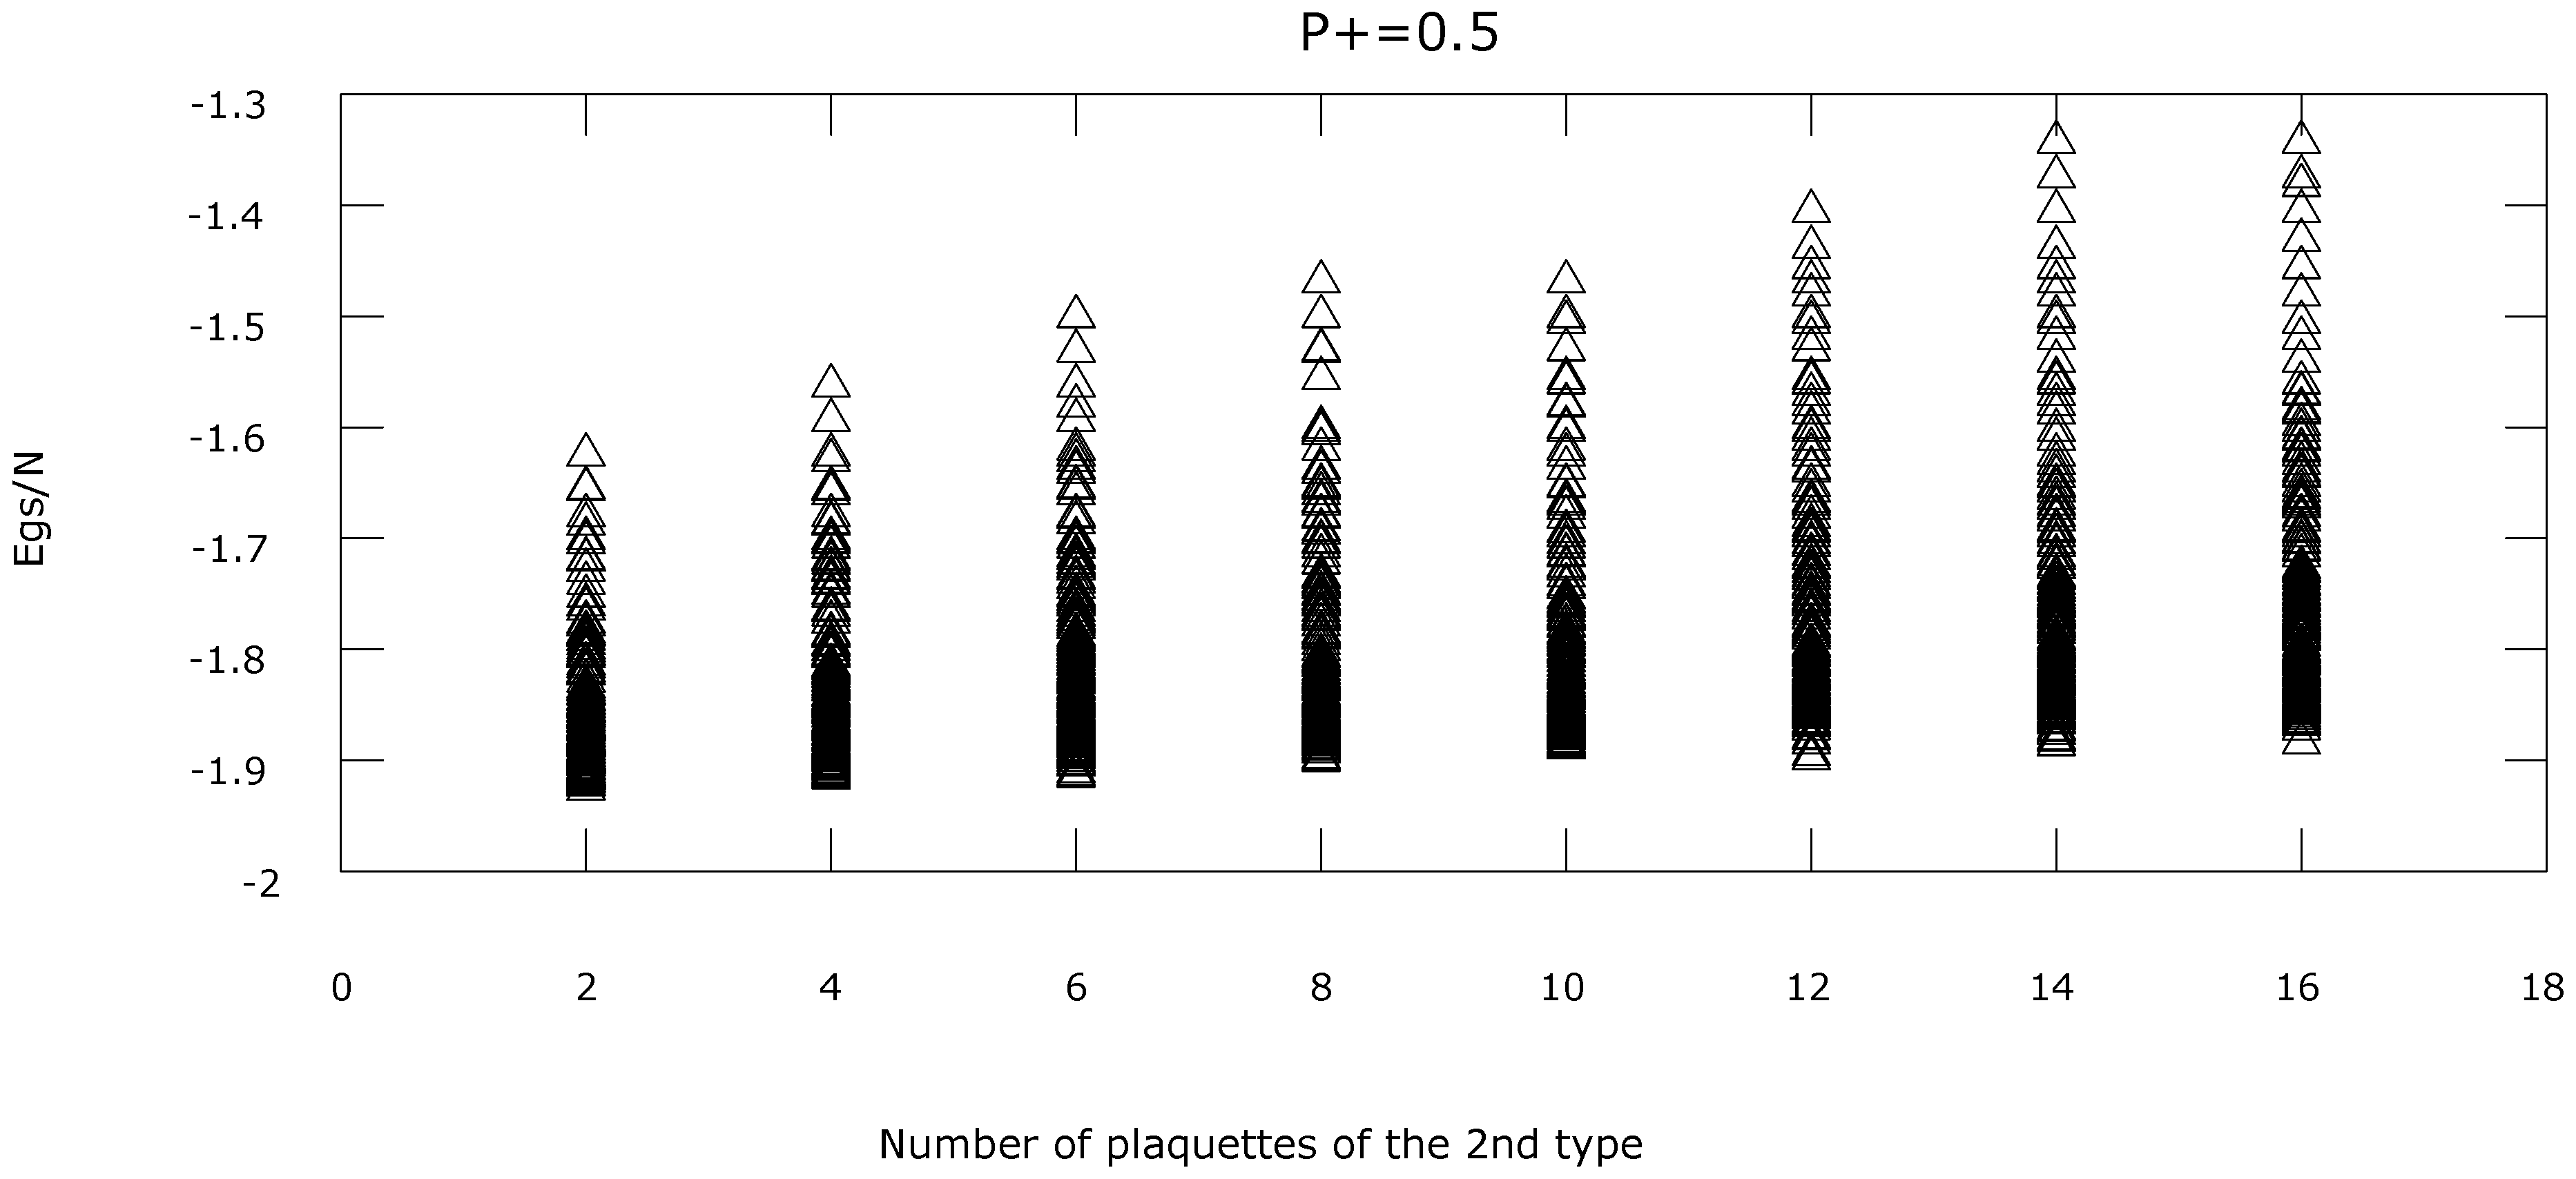
\includegraphics{Egs_N_F.eps}}
	\caption{Зависимость энергии основного состояния на один спин от количества фрустрированных плакетов}
	\label{fig:Egs_N_F}
\end{figure}

Из графика \ref{fig:Egs____N_F} видно, что системы обладающие одинаковым количеством фрустрированных плакетов распологаются на одних и тех же линиях. Чем меньше угол между линией и осью ординат, тем больше фрустрированных плакетов в системах находящихся на этой линии. Таким образом, зная размеры системы и посчитва количество фрустрированных плакетов не состваит труда воспользовавшись графиком найти энергию основного состояния.

\begin{figure}[H]
	\centering
	\resizebox{290px}{220px}{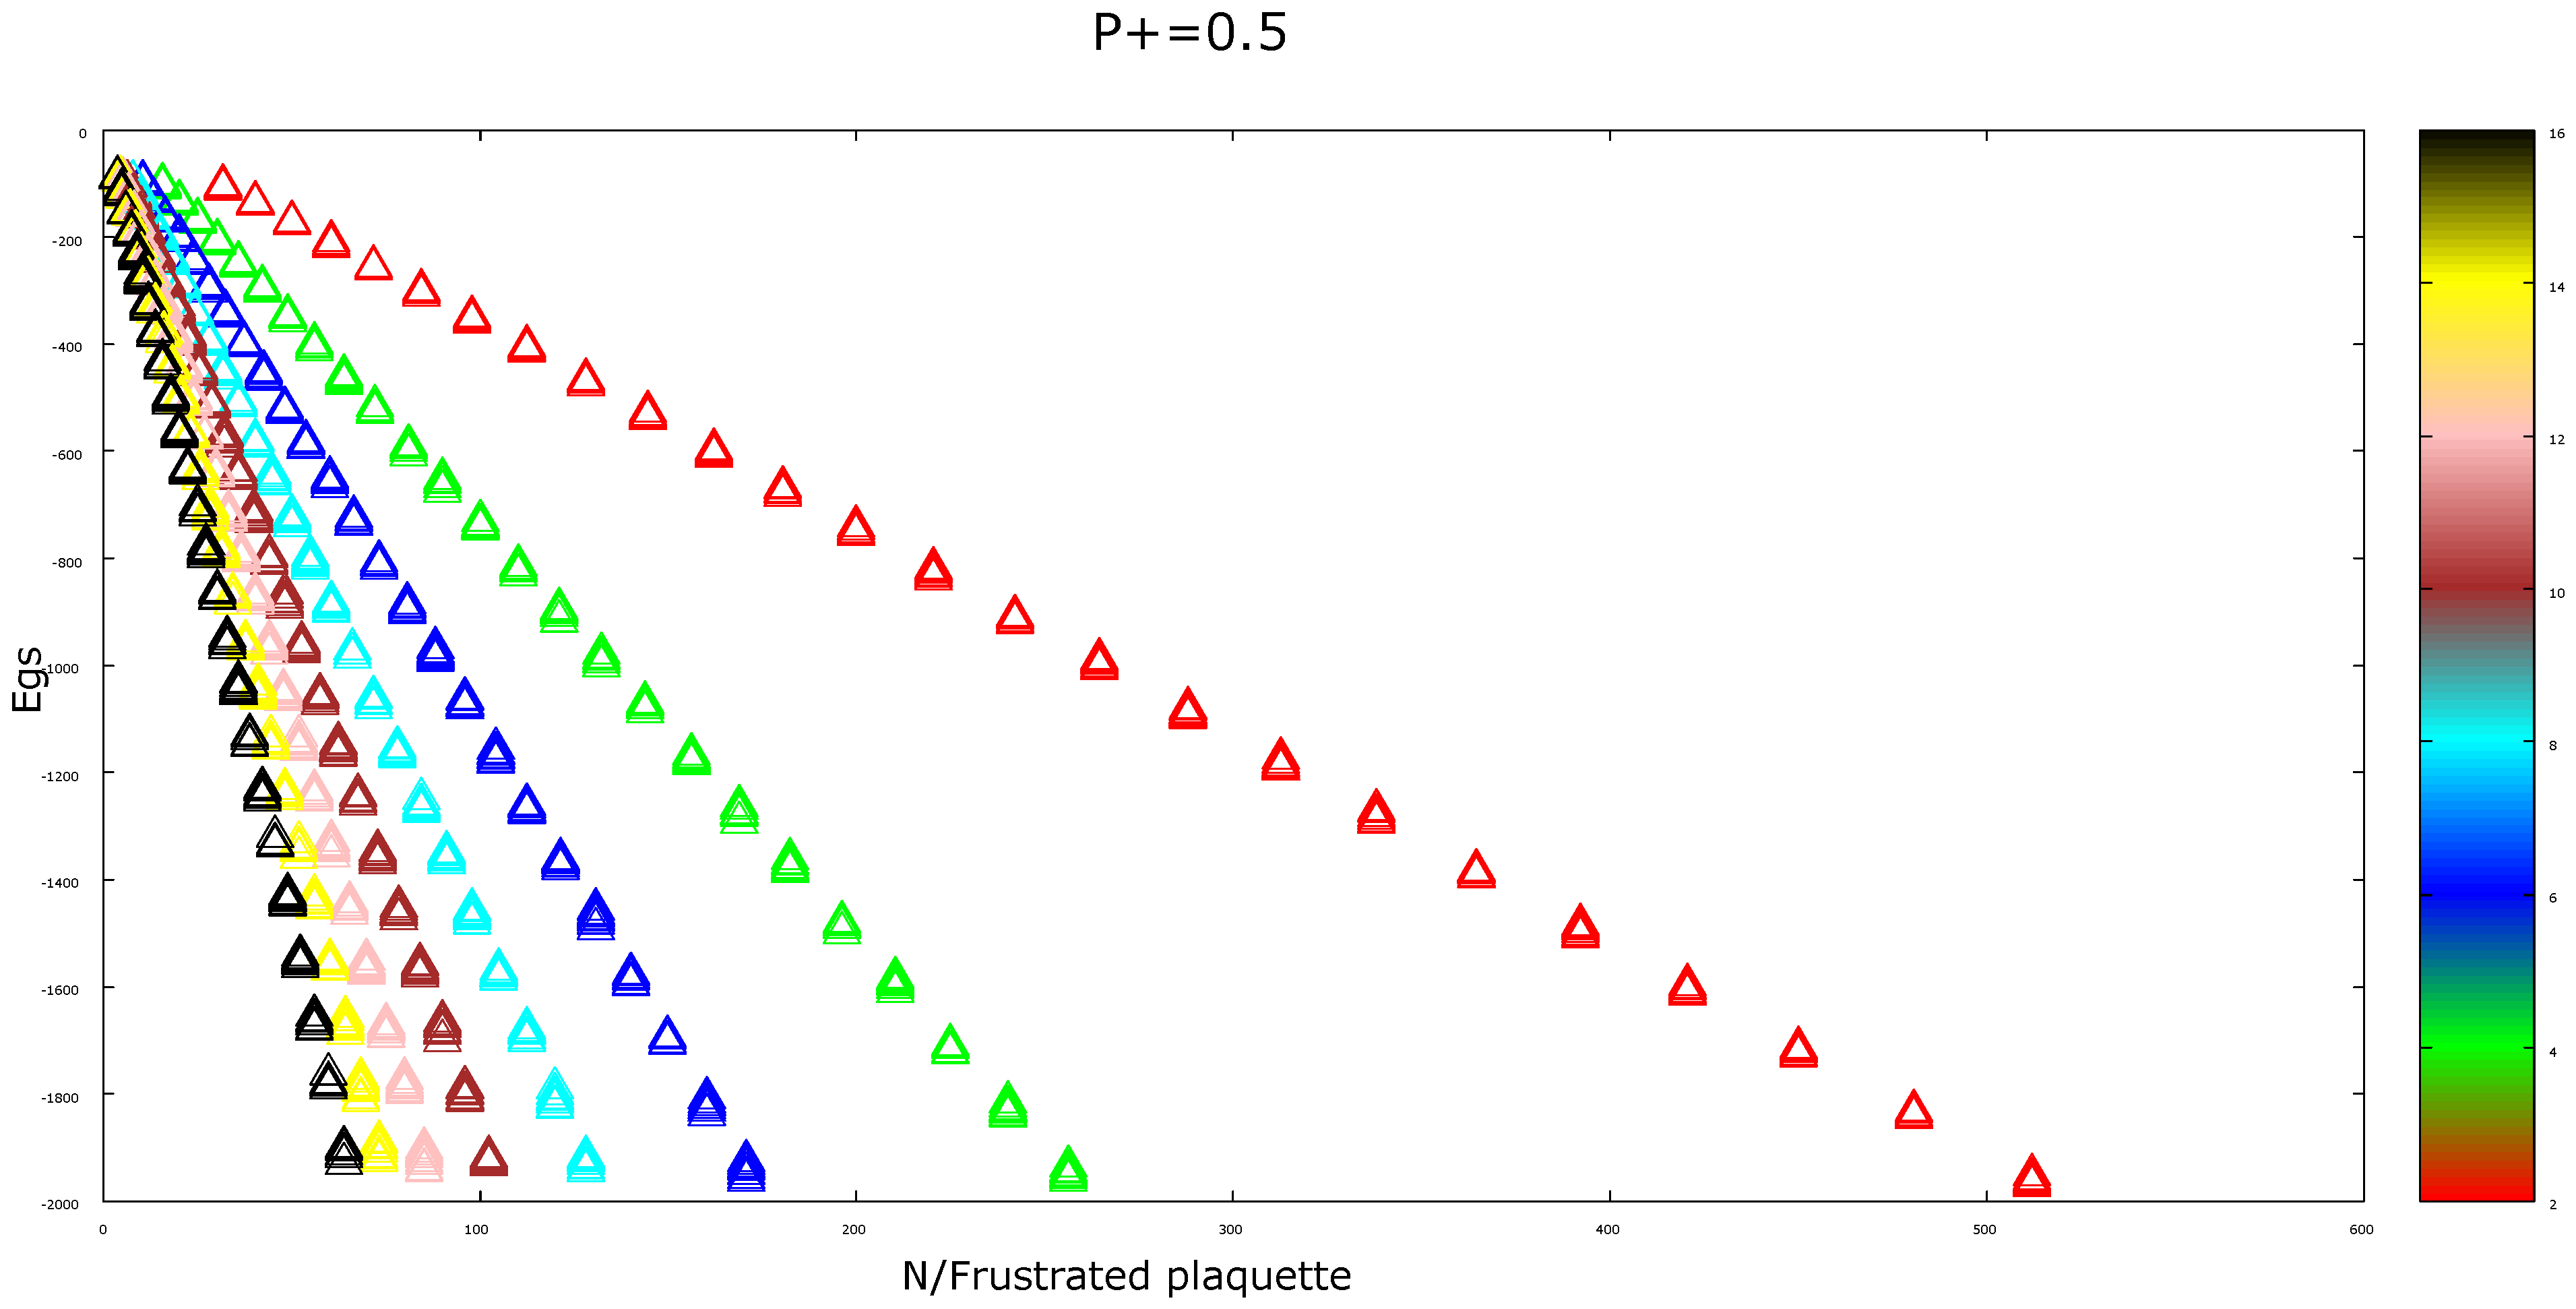
\includegraphics{Egs____N_F.eps}}
	\caption{Зависимость энергии основного состояния от количества спинов на один фрустрированный плакет}
	\label{fig:Egs____N_F}
\end{figure}

\section{Заключение}

С помощью разработанных программ ЭВМ на основании авторского подхода, а также с помощью известных методов возможно проведение исследований основных состояний фрустрированных спиновых моделей на решетках, расчет фазовой диаграммы в отсутствии температуры, исследование возбуждений и макроскопического вырождения основного состояния в зависимости от поля, поведения спинового избытка, конфигураций основного состояния во внешнем магнитном поле для развития физики конденсированного состояния.


\section{Благодарности}

 

\bibliography{mybibfile}


\end{document}